\documentclass[runningheads,a4paper]{llncs}
\usepackage[utf8]{inputenc} % allow utf-8 input
\usepackage{amssymb}
\setcounter{tocdepth}{3}
\usepackage{graphicx}
\usepackage{multirow}
\usepackage{algorithm}
\usepackage{algpseudocode}  % para pseudocodigo
%\input{algorithmic} % mi archivo de traducción

\usepackage{url}
\urldef{\mailsa}\path|francomorero96@gmail.com|    
\urldef{\mailsb}\path|saltoc@ing.unlpam.edu.ar|    
\newcommand{\keywords}[1]{\par\addvspace\baselineskip
\noindent\keywordname\enspace\ignorespaces#1}

\begin{document}

\mainmatter  % start of an individual contribution

% first the title is needed
\title{A Simple Differential Evolution Algorithm to Solve the Flexible Job Shop Scheduling Problem}

% a short form should be given in case it is too long for the running head
\titlerunning{DE for the FJJSP}


\author{Franco Morero  \and Carlos Bermudez \and Carolina Salto }

\institute{Facultad de Ingeniería, UNLPam\\
General Pico, La Pampa, Argentina, CONICET\\
%\mailsa 
%\mailsb\\
}


\maketitle


\begin{abstract}
This paper addresses the Flexible Job Shop Scheduling Problem (FJSSP) where the objective is to minimize the makespan. We develop a parallel hybrid Differential Evolution (DE) algorithm to tackle this problem. A random key representation of the FJSSP is adopted, which requires a very simple conversion mechanism to obtain a feasible schedule. This allows the DE algorithm to work on the continuous domain to explore the problem space of the discrete FJSSP. Moreover, a simple local search algorithm is embedded in the DE framework to balance the exploration and exploitation by enhancing the local searching ability. In addition, parallelism of the DE operations is included to improve the efficiency of whole algorithm. Experiments confirm the significant improvement achieved by integrating the propositions introduced in this study. Additional, test results show that our algorithm is competitive when compared with most existing approaches for the FJSSP. 
\keywords{flexible job shop scheduling, differential evolution algorithm, parallelism}
\end{abstract}


\section{Introduction}
\vspace{-0.4cm}
%Hablar sobre DE, que todos sus operadores están pensados para reales. 
%Resolver el problema FJSSP utilizando una representación basada en reales lo cual implica una aplicación directa del DE sin necesidad de utilizar operadores específicos para otras representaciones que pueden complicar o bien alejar la concepción básica del DE

%hacer un pequeño estado del arte de soluciones del FJSSP utilizando DE haciendo hincapié en la representación adoptada. Incluir el trabajo de los chicos (creo)

%Mencionar las ventajas del paralelismo en la resolución de un problema y de las formas posibles de incorporar paralelismo, la adoptada en este trabajo.

%detallar objetivo del trabajo, metodología/contribuciones.

%organización del trabajo.

%Some of the real-life optimization problems cannot be tackled by exact methods which would be implemented laboriously and in a time-consuming manner. For such optimization problems, metaheuristics are used with less computational effort to find good solution from a set of large feasible solutions. One example of this kind of problems is the scheduling problem. There are a considerable amount of efforts devoted to solve this problem, explained not only by the fact that most of the problems in the family of scheduling are computationally hard~\cite{Pinedo:2008:STA:1477600} and therefore there is still room for improvement in the resolution methods, but also because manufacturing and production are continuously changing and introducing more and more demanding restrictions.

%The Job Shop Scheduling Problem (JSSP) is one of most important and difficult problems~\cite{Pinedo:2008:STA:1477600} in the scheduling problem family. Each job has to undergo multiple operations on the various machines. The decision concerns how to sequence the operations on the machines, so that the time needed to complete all the jobs (makespan) is minimized. The possibility of selecting alternative routes among the machines is useful in production environments where multiple machines are able to perform the same operation (possibly with different processing times), as it allows the system to absorb changes in the demand of work or in the performance of the machines. When this factor is considered, the problem is known as Flexible Job Shop Scheduling Problem (FJSSP).

%One example of 
A realistic production environment, and with practical applicability, is the Flexible Job Shop Scheduling Problem. Each job has to undergo multiple operations on the various machines. The decision concerns how to sequence the operations on the machines, so that the time needed to complete all the jobs ($C_{max}$) is minimized. Moreover, an additional decision consists in to assign each operation to the appropriate set of machines. These decisions suggest that the FJSSP is a complex optimization problem (NP-hard problem~\cite{Garey:1976:CFJ:2782828.2782830}), %the adoption of heuristic methods is suggested because they produce reasonably good schedules in a reasonable time, instead of looking for an optimum solution, also for small instances. In recent years, 
consequently, the adoption of metaheuristic~\cite{Talbi,Luque:2013:PGA:2564896} has led to better results than classical dispatching or greedy heuristic algorithms~\cite{tang2011,Wang2012917,WANG2017}. %\cite{Mastrolilli1996,Pezzella20083202,Vilcot2008398,Zhang20091309,Zhang2011}.
Since introduced in 1997 by Storn and Price~\cite{Storn1997}, the Differential Evolution (DE) metaheurisitc became very popular among computer scientists and practitioners almost immediately after its original definition. 

DE is a stochastic real-parameter global optimizer. It employs simple mutation and crossover operators to generate new candidate solutions, and applies one-to-one competition scheme to greedily determine whether the new candidate or its parent will survive in the next generation. Their successful is due to its simplicity and ease implementation, and reliability and high performance. DE algorithms have been applied to many combinatorial optimization problems 
%, ranging from Scheduling Problems [3] to routing vehicles~\cite{MINGYONG2010188,Teoh:2015:DE-CVRP}. Moreover, DEs have been applied for solving structural optimization problems~\cite{GRECO20191,Hull:DE-StructuralOpt}, for parameter/tolerance design problems~\cite{Rout2010}, and health monitoring (Casciati, 2008), among many others. 
(\cite{%MINGYONG2010188,
Teoh:2015:DE-CVRP,GRECO20191,Hull:DE-StructuralOpt,Rout2010}, among many others), but as far as we are aware, there is few published research work that describes the use of DE to deal with the FJSSP~\cite{YUAN2013246}. 


In this work, a simple DE to solve the FJSSP is design. As DE was originally devised for solving continuous optimization problems, we adopt a real value representation for the FJSSP  to make the continuous DE applicable for solving the discrete FJSSP, which implies that algorithm operations should not be modified or adapted to resolve the problem. Another important feature of DE is the little number of parameters to be set, when compared to other evolutionary algorithms%: with only three parameters, the algorithm behaviour can be controlled
. However, the success to find good solutions to a problem depends on discovering the correct values of those parameters~\cite{%Nero2010,
app8101945}. Therefore, we make an analysis in this line to determine the adequate values for these parameters for solving the instances of the FJSSP. Moreover, a simple local search procedure is embedded to the DE to improve their exploration capacities by solving the problem. Finally, parallelism at algorithmic level~\cite{Talbi} is incorporated to the design of the DE, with the aim of improving the scalability and reducing the computation time.  %Therefore, the contributions of this work are:
%\begin{itemize}
%\item design of a simple DE to solve the FJSSP in the real-value search space,
%\item improvement of the DE with a simple and efficient local search procedure,
%\end{itemize}
The experimental methodology we have followed consists of computing the $C_{max}$ values for the different DE proposed to solve the FJSSP and then comparing the obtained results by considering different quality indicators. We find that our simple DE shows a promising behavior to solve the FJSSP.% when compared to other metaheuristics of the literature.

The  paper is organized as follows. In Section~\ref{sec:FJSSP}, we introduce the problem formulation %and show an illustrative example of input data
.  In Section~\ref{sec:DE}, we present the basic DE algorithm. In Section~\ref{sec:HDE} we explain the adaptations of the DE to solve the FJSSP. In the following section, we introduce the experimental design and in Section 6, we evaluate the results. %Further, in Section 6 we make a comparison between these metaheuristics and the ones present in the literature. 
Some final remarks and future research directions are given in Section 7.

\section{The Flexible Job Shop Scheduling Problem} \label{sec:FJSSP}
\vspace{-0.4cm}
The FJSSP can be formally described as follows. A set $J = \{J_1, J_2, . . . , J_n\}$ of independent jobs and a set $U = \{M_1,M_2, . . . , M_m\}$ of machines are given. A job $J_i$ is broken down by a sequence of $O_{i1},O_{i2}, . . . , O_{in_i}$ operations to be performed one after the other according to the given sequence. Each operation $O_{ij}$ can be executed on any among a subset $U_{ij} \subseteq U$ of compatible machines. We have partial flexibility if there exists a proper subset $U_{ij} \subset U$, for at least one operation $O_{ij}$, while we have $U_{ij} =U$ for each operation $O_{ij}$ in the case of total flexibility. The processing time of each operation is machine-dependent. We denote with $d_{ijk}$ the processing time of operation $O_{ij}$ when executed on machine $M_k$. Pre-emption is not allowed, i.e., each operation must be completed without interruption once started. Furthermore, the machines cannot perform more than one operation at a time. All jobs and machines are available at time 0.

The problem is to assign each operation to an appropriate machine (routing problem), and to sequence the operations on the machines (sequencing problem) in order to minimize the makespan ($C_{max}$). This measure is the time needed to complete all the jobs, which is defined as $C_{max} = max_i\{C_i\}$, where $C_i$ is the completion time of job $J_i$.  Table~\ref{tab:proccesingTime} shows an instance of the FJSSP with 3 jobs, 4 machines and 8 operations. The rows and columns correspond to machines and operations, respectively, and the entries of the table are the processing times. %In this example, we have a partial flexible scenario, an ``$-$'' entry in the table means that a machine cannot execute the corresponding operation, i.e., it does not belong to the subset of compatible machines for that operation. %According to the evolution paradigm used in GAs, we will refer to any solution of FJSP as an individual or chromosome.

% \begin{table}[tb]
% \scrptsize
%   \centering
%   \caption{Instance Example for the FJSSP}
%     \begin{tabular}{ccrrrr}
%    \hline
%           & & $M_1$    & $M_2$    & $M_3$    & $M_4$ \\ \hline
%     \multirow{3}[0]{*}{$J_1$} & $O_{11}$   & --     & 6     & 5     & -- \\
%     & $O_{12}$   & 4     & 8     & 5     & 6 \\
%     & $O_{13}$   & 9     & 5     & -     & 7 \\\hline
%     \multirow{3}[0]{*}{$J_2$} & $O_{21}$   & 2     & -     & 1     & 3 \\
%     & $O_{22}$   & 4     & 6     & 8     & 4 \\
%     & $O_{23}$   & 9     & -     & 2     & 2 \\\hline
%     \multirow{2}[0]{*}{$J_3$} & $O_{31}$   & 8     & 6     & -     & 5 \\
%     & $O_{32}$   & 3     & 5     & 8     & 3 \\ \hline
%     \end{tabular}%
%   \label{tab:proccesingTime}%
% \end{table}%

\begin{table}[tb]
\scriptsize
   \centering
   \caption{Instance Example for the FJSSP}
   \label{tab:proccesingTime}%
\begin{tabular}{c|ccc|ccc|cc}
\hline
\multicolumn{1}{l|}{} & \multicolumn{3}{c}{$J_1$} & \multicolumn{3}{c}{$J_2$} & \multicolumn{2}{c}{$J_3$} \\
\hline
\multicolumn{1}{l|}{} & $O_{11}$    & $O_{12}$   & $O_{13}$   & $O_{21}$    & $O_{22}$   & $O_{23}$   & $O_{31}$        & $O_{32}$       \\
\hline
$M_1$                   & -      & 4     & 9     & 2      & 4     & 9     & 8          & 3         \\
$M_2$                   & 6      & 8     & 5     & -      & 6     & -     & 6          & 5         \\
$M_3$                   & 5      & 5     & -     & 1      & 8     & 2     & -          & 8         \\
$M_4$                   & -      & 6     & 7     & 3      & 4     & 2     & 5          & 3        \\
\hline
\end{tabular}
\end{table}
 %problem description

\section{Differential Evolution Algorithm: Background}
\label{sec:DE}
\vspace{-0.4cm}
The DE algorithm was proposed by Storn and Price~\cite{Storn1997} to solve optimization problems with real-valued parameters. DE is a stochastic, population-based  optimization method. Despite having a very simple algorithmic structure, DE has demonstrated a high level of performance when solving a wide variety of very complex problems~\cite{Price:2005}. The optimal or near-optimal solution is obtained by an iterative process which is applied to a set of solutions (population) to achieve a new one. At each step of the process, new solutions arise as a result of perturbations to the current solutions, caused by mutation and recombination operators. %The general structure of the DEA shares similar features with other evolutionary algorithms, such as genetic algorithm (GA)~\cite{holland75}. DE algorithm is different in handling distance and direction information to move the population at the current generation toward the next generation, in virtue of a constructive cooperation between individuals.

The algorithmic framework of DE is described in Algorithm~\ref{alg:algoritmoDE}. The first step (Line 1) consists in the initialization of the population $P^0$ of $N_P$ target vectors of \textit{D} real values ($x_i = (x_{i,1}, x_{i,2}, . . . , x_{i,D}) \in \mathbb{R}^{D}  (1 \leq i \leq N_P)$). Each component $x_{i,j} \in \mathbb{R} (1 \leq j \leq D)$ represents a variable or a parameter of the optimization problem. Usually, each $x_{i,j}$ is bounded to a value in the range $[li_j, ls_j]$, where $li_j$, $ls_j \in \mathbb{R}$ are the lower and upper bound, respectively. The $N_P$ target vectors are initialized randomly by applying Equation~\ref{eqDE:Init}:
\vspace{-0.2cm}
\begin{equation}\label{eqDE:Init}
x_{i,j} = li_{j} + U(0, 1) \times (ls_j - li_j)
\end{equation}
%\vspace{-0.1cm}
\noindent where $U(0, 1)$ is a random number with uniform distribution in the range $[0, 1]$. 

\begin{algorithm}[tb]
\scriptsize
    \caption{Differential Evolution Algorithm (DE)} \label{alg:algoritmoDE}
    \begin{algorithmic} [1]
    \Require {$F, Cr, N_p$} 
    \Ensure {$x_{best}$} 
        \State initialize($P^0$,$N_p$) 
        \State $g \leftarrow 0$
        \While {not meet stop criterion}
            \For {each vector $x_{i}^g$ from $P^g$}
                \State $v_{i}^g \leftarrow $ mutate($x_{i}^g, P^g, F$) 
                \State $u_{i}^g \leftarrow $ recombinate($x_{i}^g, v_{i}^g, Cr$)
                \State $x_{i}^g \leftarrow $ select($x_{i}^g, u_{i}^g$)
                \State add($P^{g+1}, x_{i}^{g+1}$) 
            \EndFor
            \State $g \leftarrow g+1$ 
        \EndWhile
        \State$x_{best} \leftarrow $best\_solution($P^{g}$)
    \end{algorithmic}
\end{algorithm}


%After the initialization step, an iterative process begins, which consists in the application of mutation (Line 5 of Algorithm~\ref{alg:algoritmoDE}), recombination (Line 6), and selection (Line 7) operations until an stop criterion is reached. 

After the initialization step, an iterative process begins. The mutation operation (Line 5 of Algorithm~\ref{alg:algoritmoDE}) obtains a donor vector $v_i^g = (v_{i,1}, v_{i,2}, . . . , v_{i,D})$ for each target vector $x_i^g$ from the current population $P^g$ ($0 \leq g \leq max_{gen}$) following Equation~\ref{eqDE:mutation}. To obtain $v_i^g$, a base vector $x_{r0}^g$ and other two vectors $x_{r1}^g$ y $x_{r2}^g$ are randomly selected from $P^g$, with $r0, r1$ and $r2$ chosen from the set $\{1,2,...,N_P\}$ and all of them are mutually exclusive. The $F \in [0 . . . 1)$ factor, known as scale factor, controls the rate at which the population evolves, in order to avoid their stagnation during the search process. The mutation operator is important to the DE's behaviour because it focuses the search on the most promising areas of the solution space. 
\vspace{-0.1cm}
\begin{equation}\label{eqDE:mutation} 
v_i^g = x_{r0}^g + F \times (x_{r1}^g - x_{r2}^g)
\end{equation}
%\vspace{-0.4cm}
The donor vector is modified by the recombination operator (Line 6), with the aim of increasing the population diversity. This operator creates a trial vector $u_i^g$ through mixing components of the donor vector $v_i^g$ and the target vector $x_i^g$. The most frequently referred crossover operator is the binomial crossover, which is shown in Equation~\ref{eqDE:recombination}:
\vspace{-0.4cm}
\begin{equation} \label{eqDE:recombination}
u_{i,j}^g = \left\lbrace
\begin{array}{ll}
v_{i,j}^g & \textup{si } r_j < Cr \vee j = j_r\\
x_{i,j}^g & \textup{otherwise} 
\end{array}
\right.
\end{equation}
%\vspace{-0.4cm}
\noindent where $r_j=U(0, 1)$ is a random value, $j_r$ is also a random value in the set \{1, 2, ...,$D$\}, and finally $Cr$ is a parameter known as recombination probability, which controls the fraction of parameter values that are copied from the donor.

The last step %in the DE's iterative process 
is the selection operation (Line 7). The trial vector $u_{i}^g$ competes against the target vector $x_{i}^g$ regarding their objective values (obtained applying the objective function to each vector). The best vector is selected to be part of the population $P^{g+1}$ of the next generation%(see the Equation~\ref{eqDE:selection})
. Clearly, this competition %between parents and children 
creates a new population with a performance equal or superior to the current one (Line 8). Consequently, DE is an elitist evolutionary algorithm. 

%\begin{equation} ~\label{eqDE:selection}
%x_{i}^{g+1} = \left\lbrace
%\begin{array}{ll}
%u_{i}^g & \textup{if } f(u_{i}^g) \textup{ \textit{ is equal or best than} } f(x_{i}^g)\\
%x_{i}^g & \textup{otherwise} 
%\end{array}
%\right.
%\end{equation}

The stopping criteria can be set to a preset maximum number of iterations ($max_{gen}$) or some other problem-dependent criterion. Whichever the criteria to be set, the choice has a direct influence on the best solution $x_{best}$ obtained by the algorithm (Line 12). 

DE performance mainly depends on three parameters: scaling factor of the difference vector ($F$), crossover control parameter ($Cr$) and population size ($N_P$). Some guidelines are available to choose the control parameters~\cite{Price:2005}. In this work, $N_P$ and $F$ are chosen  based  on  previous  knowledge  and  keep  it  constant during all runs. % The factor $F$ usually takes a value that ranges from 0.4 to 1.0~\cite{Gamperle02aparameter}. 
On the other hand, a good value for $Cr$ is 0.1 however, to speed up convergence a greater value can be used. %DE description

\section{Our proposal: Hybrid DE for the FJSSP}
\label{sec:HDE}
\vspace{-0.2cm}
In this section, our proposal to solve the  FJSSP is detailed. In order to apply the DE algorithm, it is crucial to design a suitable encoding scheme that maps the floating point vectors to the feasible solution for the FJSSP (see Section~\ref{subsec:rep}). Moreover, our proposal is enhanced by a simple local search (Section~\ref{subsec:HDE}). Finally, a parallel version of our proposal is introduced (Section~\ref{subsec:parallelHDE}).


\subsection{Representation}  \label{subsec:rep}
\vspace{-0.25cm}
In this work, the DE algorithm still manipulates real-valued vector in order to maintain the simplicity and properties of the DE in their natural configuration. Consequently, the schedule is generated following the random keys encoding scheme~\cite{Bean1994RepRandomKeys}. This representation deals with real point vectors, where these points are used as sort keys to decode the solution. For an $n$-job $m$-machine scheduling problem, each vector's position (a random key) consists of a floating number in U(-1,1) which can be translated to an unique list of ordered operations, after a descending order of the random keys. These steps always obtain a feasible schedule from a real-valued vector. The schedule is a permutation with repetitions~\cite{bierwirth1995}. See Figure~\ref{fig:decodificacion} for an example considering the instance shown in Table~\ref{tab:proccesingTime}. Given the vector $x_i^g$=[0.6,-0.5,0.4,-0.3,-0.1,0.9,-0.7,0.2], it is converted to a schedule $[2, 1, 1, 3, 2, 2, 1, 3]$, which is a permutation of the set of operations that represents a tentative ordering to schedule them, each one being represented by its job number. This valid schedule corresponds to the operation sequence $O_{21}$, $O_{11}$, $O_{12}$, $O_{31}$, $O_{22}$, $O_{23}$, $O_{13}$, and $O_{32}$. 

In order to evaluate $x_i^g$, the objective value is the makespan ($C_{max}$). To compute it, each operation $O_{ij}$ in $x_i^g$ is assigned to a feasible machine $M_k$ in $U_{ij}$ with the shortest completion time, and then the load of $M_k$ must be updated. The initial solution is generated by a random procedure (Equation 1), mainly because high performing construction heuristics for the FJSSP are unknown.
%
%The decoding procedure is explained in Algorithm~\ref{alg:algoritmoDecodificacion} and is applied before the evaluation of an vector begins. An illustrative example is shown in FigureXX.
%
%En la figura \ref{fig:decodificacion} se puede ver un ejemplo de este procedimiento para una instancia del problema FJSSP con 3 trabajos, 4 máquinas y 8 operaciones mostrada en la tabla
%
\begin{figure}[tb]
    \centering
    
\includegraphics[width=0.55\textwidth]{./figures/deco.eps}
    \caption{Example of the decoding process used by the DE to solve the FJSSP.}
    \label{fig:decodificacion}
    \vspace{-0.4cm}
\end{figure}
%
\subsection{DE and Local Search Method} \label{subsec:HDE}
\vspace{-0.25cm}
DE is enhanced with a local search technique, yielding a hybrid DE (HDE) for exploration and exploitation among the solutions to obtain a near optimal solution. In this work, a simple interchange mechanism is implemented in which two positions of the target vector are randomly selected  and interchanged. If there is an improvement in the objective function the swap is accepted, otherwise, it is not considered. %The pseudo-code of local search procedure is given in Figure~\ref{alg:algoritmoLS}. 
This local search procedure is applied to the target vectors $x_{i}$ of the next population (just before Line 11 of Algorithm~\ref{alg:algoritmoDE}) but not to the trial vector $u_{i}$, which is beneficial to avoid both cycling search and getting trapped in a local optimum. Moreover, the frequency of the local search is controlled by the probability $p_{LS}$. Another important characteristic of this local search procedure is that it does not need a backward conversion because it is applied over the real-valued vector.
%
%
%Con el fin de mejorar la eficiencia de DE, se incorporó al algoritmo un procedimiento de busqueda local, que actua sobre la población justo antes de la línea 10 del algoritmo \ref{alg:algoritmoDE}. En el algoritmo \ref{alg:algoritmoLS} se puede ver un pseudocodigo del proceso realizado, el cual consiste en iterar sobre todos los individuos de la población, obtener un número aleatorio y si es menor a una probabilidad de aplicar busqueda local realizar las siguientes acciones: seleccionar 2 indices aleatorios en el individuo $x_{i}$, intercambiar entre ellos obteniendo un nuevo vector de prueba $u_{i}$, y si al evaluar $u_{i}$ obtenemos una solución igual o mejor que $x_{i}$, seleccionar $u_{i}$ como nuevo individuo de nuestra población.
%
%\begin{algorithm} [H]
%    \caption{Local Search Procedure} \label{alg:algoritmoLS} 
%    \begin{algorithmic} [1]
%        \For {each $x_{i}^g$ from $P^{g}$}
%            \If {$random() < PBL$} %\Comment PBL: probabilidad de busqueda local
%                \State $j$ , $k \leftarrow $ random(1,$D$)
%                \State $u_{i} \leftarrow $ swap($x_{i}$, $j$,$k$)
%                \If {$f(u_{i}) \leq  f(x_{i})$} \Comment{for a minimization problem}
%                    \State $x_{i} \leftarrow u_{i}$
%                \EndIf
%            \EndIf
%        \EndFor
%    \end{algorithmic}
%\end{algorithm}

\subsection{DE and Parallelism} \label{subsec:parallelHDE}
\vspace{-0.2cm}
In terms of designing parallel metaheuristics, the DE can be paralleled in different ways~\cite{Talbi}. %For instance, their population-based characteristics allow evaluating in a parallel way the fitness value of each individual, giving rise a global or master-slave model. In this same line, each iteration of a metaheuristic can be parallelized. In this two cases, the behaviour of the metaheuristic is not altered. Parallelism can also be exploited to perform the genetic operators in a semi-isolated manner, resulting in the island model. Finally, the previous strategies can be combined, giving rise to the cellular model~\cite{albaPEA2006}. This last two models alter the behavior of the metaheuristic and enable the improvement of the quality of solutions.
In this work, the aim of the parallelization is not to change the behaviour of the metaheuristic but to speed up the search. For that purposes, we focus on the parallelization of each iteration of the DE~\cite{albaPEA2006}. The population of individuals is decomposed and handled in parallel, using the well-known global parallelization model. A principal process performs the selection operations and the replacement, which are generally sequential. The rest processes (workers) perform the mutation, recombination, and the evaluation of the solutions in parallel. Consequently, this model maintains the sequence of the original algorithm, and hence the behavior of the metaheuristic is not altered. 








%Actuando sobre la eficiencia del algoritmo, con el fin de mejorar la velocidad del mismo, se optó por un esquema de ejecución en paralelo. Teniendo en cuenta que a cada individuo se lo trata por separado en el proceso de evolución, se cosideró realizar estas ejecuciones en paralelo, tomando cantidades iguales de individuos de la poblacion y asignando cada parte a unidades de procesamiento diferentes. La misma idea se tomo para mejorar la eficiencia en la búsqueda local, otorgando grandes ventajas en cuanto a velocidad y aprovechamiento de recursos.

%\subsection{Implementación de \textit{DE} híbrido para \textit{FJSSP}}
%El algoritmo \ref{alg:algoritmoDEhibrido} presenta el pseudocodigo del algoritmo de \textit{DE} hibrido para \textit{FJSSP}. Como se puede observar el esquema general es el mismo que el presentado anteriormente, con la inclusión del proceso de búsqueda local. Además, se agrega como entrada la probabilidad de aplicar busqueda local ($PBL$).

%\begin{algorithm} [H]
%    \caption{Pseudocodigo de la Evolucion Diferencial (DE)} \label{alg:algoritmoDEhibrido}
%    \begin{algorithmic} [1]
%    \Require {$F, Cr, N_p, PBL$} 
%    \Ensure {$x_{best}$} 
%        \State inicializar($P$,$N_p$) 
%        \State $g \leftarrow 0$
%        \While {no se alcance la condición de fin}
%            \For {cada vector $x_{i}^g$ de $P^g$}
%                \State $v_{i}^g \leftarrow $ mutacion($x_{i}^g, P^g, F$) 
%                \State $u_{i}^g \leftarrow $ recombinacion($x_{i}^g, v_{i}^g, Cr$)
%                \State $x_{i}^g \leftarrow $ seleccion($x_{i}^g, u_{i}^g$)
%                \State agregar($P^{g+1}, x_{i}^{g+1}$) 
%            \EndFor
%            \State busqueda-local($P^g$, $PBL$)
%            \State $g \leftarrow g+1$ 
%        \EndWhile
%        \State$x_{best} \leftarrow $mejor-solucion($P^{g}$)
%
%    \end{algorithmic}
%\end{algorithm}



 %DE description

\section{Experimental Design} \label{sec:experDesig}

In this section, we describe the experimental design followed in this approach. We have selected a wide range of FJSSP instances used in the literature taking into account their complexity, which is given by the number of jobs and machines, and the wide variation of flexibility in the number of available machines per operation. In this sense, we considered the data set proposed by Brandimarte~\cite{brandimarte1993} as a representative one. The number of jobs ranges from 10 to 20, the number of machines belongs to the set \{4,15\} and the number of operations for each job varies from 5 to 15. Consequently, the total number of operations ranges from 55 to 240. The flexibility is between 1.43 and 4.10.

Concerning the methodology followed to analyze the results, first, we studied the behavior of these algorithms with different $F$ and $Cr$ values, considering the best $C_{max}$ found and the number of iterations to reach them for each instance. This analysis allows us to determine the best values for the control parameters. Secondly, we determined the impact of incorporating a local search procedure at different rates of $p_{LS}$. For this purpose, we take into account the best $C_{max}$ found, and the number of iterations to reach the best solution for each instance. Finally, we study DE's behaviour including parallelism regarding the execution time of each approach. The analyses are principally validated by the data in the tables and figures shown in the experimental research section.

The parametric configuration considered for DE's experimentation is the following. The population size $N_P$ is set to 50. The $F$ factor and the $Cr$ probability are tested with three different values (0.1, 0.5, and 0.9). For the remaining parameter, $p_{LS}$, three values are also analysed (0.1, 0.5 and 0.7). Table~\ref{tab:parameteres} shows a summary of the parameters.

\begin{table}[tb]
\scriptsize
\centering
\caption{Parameter Values}
\begin{tabular}{cc}
\hline
\multicolumn{1}{c}{Parameter} & \multicolumn{1}{c}{Values} \\ 
\hline
NP                              & 50                          \\
F                               & 0.5, 0,7, and 0,9           \\
Cr                              & 0.1 and 0.9                 \\
$p_{LS}$                          & 0.5, 0,7, and 0,9          \\
\hline
\end{tabular}
\label{tab:parameteres}
\end{table}
%
\begin{table*}[!tb]
    \scriptsize
  \centering
  \caption{Best values of $ C_{max} $ found by the DE algorithm with different $F$ and $Cr$ values for all FJSSP instances}
    \begin{tabular}{rrccccccccc|}
    \hline
\multicolumn{1}{|c|}{} & \multicolumn{1}{c|}{} & \multicolumn{3}{c|}{\textbf{F=0.1}} & 
\multicolumn{3}{c|}{\textbf{F=0.5}} & 
\multicolumn{3}{c|}{\textbf{F=0.9}}  \bigstrut\\
    \cline{3-11}
    \multicolumn{1}{|c|}{{\textbf{Inst.}}} & \multicolumn{1}{c|}{{\textbf{Opt.}}} & \multicolumn{1}{c|}{\textbf{Cr=0.1}} & \multicolumn{1}{c|}{\textbf{Cr=0.5}} & \multicolumn{1}{c|}{\textbf{Cr=0.9}} & \multicolumn{1}{c|}{\textbf{Cr=0.1}} & \multicolumn{1}{c|}{\textbf{Cr=0.5}} & \multicolumn{1}{c|}{\textbf{Cr=0.9}} & \multicolumn{1}{c|}{\textbf{Cr=0.1}} & \multicolumn{1}{c|}{\textbf{Cr=0.5}} & \multicolumn{1}{c|}{\textbf{Cr=0.9}} \bigstrut\\
    \hline
    \multicolumn{1}{|c|}{Mk01} & \multicolumn{1}{c|}{40} & \multicolumn{1}{c|}{\textbf{40}} & \multicolumn{1}{c|}{\textbf{40}} & \multicolumn{1}{c|}{\textbf{40}} & \multicolumn{1}{c|}{\textbf{40}} & \multicolumn{1}{c|}{\textbf{40}} & \multicolumn{1}{c|}{\textbf{40}} & \multicolumn{1}{c|}{\textbf{40}} & \multicolumn{1}{c|}{\textbf{40}} & \textbf{40} \bigstrut\\
    %\hline
    \multicolumn{1}{|c|}{Mk02} & \multicolumn{1}{c|}{26} & \multicolumn{1}{c|}{\textbf{26}} & \multicolumn{1}{c|}{27} & \multicolumn{1}{c|}{27} & \multicolumn{1}{c|}{\textbf{26}} & \multicolumn{1}{c|}{27} & \multicolumn{1}{c|}{\textbf{26}} & \multicolumn{1}{c|}{27} & \multicolumn{1}{c|}{27} & 27 \bigstrut\\
    %\hline
    \multicolumn{1}{|c|}{Mk03} & \multicolumn{1}{c|}{204} & \multicolumn{1}{c|}{\textbf{204}} & \multicolumn{1}{c|}{\textbf{204}} & \multicolumn{1}{c|}{\textbf{204}} & \multicolumn{1}{c|}{\textbf{204}} & \multicolumn{1}{c|}{\textbf{204}} & \multicolumn{1}{c|}{\textbf{204}} & \multicolumn{1}{c|}{\textbf{204}} & \multicolumn{1}{c|}{\textbf{204}} & \textbf{204} \bigstrut\\
    %\hline
    \multicolumn{1}{|c|}{Mk04} & \multicolumn{1}{c|}{60} & \multicolumn{1}{c|}{\textbf{60}} & \multicolumn{1}{c|}{\textbf{60}} & \multicolumn{1}{c|}{65} & \multicolumn{1}{c|}{61} & \multicolumn{1}{c|}{\textbf{60}} & \multicolumn{1}{c|}{\textbf{60}} & \multicolumn{1}{c|}{62} & \multicolumn{1}{c|}{63} & 62 \bigstrut\\
    %\hline
    \multicolumn{1}{|c|}{Mk05} & \multicolumn{1}{c|}{172} & \multicolumn{1}{c|}{175} & \multicolumn{1}{c|}{173} & \multicolumn{1}{c|}{173} & \multicolumn{1}{c|}{175} & \multicolumn{1}{c|}{179} & \multicolumn{1}{c|}{173} & \multicolumn{1}{c|}{175} & \multicolumn{1}{c|}{179} & 173 \bigstrut\\
    %\hline
    \multicolumn{1}{|c|}{Mk06} & \multicolumn{1}{c|}{58} & \multicolumn{1}{c|}{65} & \multicolumn{1}{c|}{59} & \multicolumn{1}{c|}{63} & \multicolumn{1}{c|}{66} & \multicolumn{1}{c|}{69} & \multicolumn{1}{c|}{59} & \multicolumn{1}{c|}{67} & \multicolumn{1}{c|}{70} & 61 \bigstrut\\
    %\hline
    \multicolumn{1}{|c|}{Mk07} & \multicolumn{1}{c|}{139} & \multicolumn{1}{c|}{143} & \multicolumn{1}{c|}{140} & \multicolumn{1}{c|}{142} & \multicolumn{1}{c|}{143} & \multicolumn{1}{c|}{148} & \multicolumn{1}{c|}{140} & \multicolumn{1}{c|}{144} & \multicolumn{1}{c|}{146} & 140 \bigstrut\\
    %\hline
    \multicolumn{1}{|c|}{Mk08} & \multicolumn{1}{c|}{523} & \multicolumn{1}{c|}{\textbf{523}} & \multicolumn{1}{c|}{\textbf{523}} & \multicolumn{1}{c|}{\textbf{523}} & \multicolumn{1}{c|}{\textbf{523}} & \multicolumn{1}{c|}{\textbf{523}} & \multicolumn{1}{c|}{\textbf{523}} & \multicolumn{1}{c|}{\textbf{523}} & \multicolumn{1}{c|}{\textbf{523}} & \textbf{523} \bigstrut\\
    %\hline
    \multicolumn{1}{|c|}{Mk09} & \multicolumn{1}{c|}{307} & \multicolumn{1}{c|}{318} & \multicolumn{1}{c|}{\textbf{307}} & \multicolumn{1}{c|}{310} & \multicolumn{1}{c|}{321} & \multicolumn{1}{c|}{333} & \multicolumn{1}{c|}{\textbf{307}} & \multicolumn{1}{c|}{321} & \multicolumn{1}{c|}{338} & \textbf{307} \bigstrut\\
    %\hline
    \multicolumn{1}{|c|}{Mk10} & \multicolumn{1}{c|}{197} & \multicolumn{1}{c|}{237} & \multicolumn{1}{c|}{210} & \multicolumn{1}{c|}{221} & \multicolumn{1}{c|}{238} & \multicolumn{1}{c|}{245} & \multicolumn{1}{c|}{206} & \multicolumn{1}{c|}{240} & \multicolumn{1}{c|}{246} & 215 \bigstrut\\
    \hline
      \multicolumn{2}{c|}{}   & 5/10 & 5/10 & 3/10 & 4/10 & 4/10 & \textbf{6/10} & 3/10 & 3/10 & 4/10 \bigstrut\\
    \cline{3-11}
    \end{tabular}%
   \label{tab:resultDE}
\end{table*}%

Because of the stochastic nature of the algorithms, we performed 30 independent runs of each test to gather meaningful experimental data and apply statistical confidence metrics to validate our conclusions. Before performing the statistical tests, we first checked whether the data followed a normal distribution by applying the Shapiro-Wilks test. Where the data was distributed normally, we later applied an ANOVA test. Otherwise, we used the Kruskal-Wallis (KW) test to assess whether or not there were meaningful differences between the compared algorithms with a confidence level of 99\%.

The considered algorithms were programmed in C++. Consequently, their runtimes are directly comparable. All algorithms were compiled on the same computer with the same compilation flags, and run on homogeneous hardware. All are positive attributes of a comparison. The experimentation is carried out on a cluster of 4 INTEL I7 3770K quad-core processors, 8 GB RAM, and the Slackware Linux with a 2.6.27 kernel version. To implement the parallel version of DE, a portable programming interface for shared memory parallel computers such us OpenMP~\cite{openMP} is used.

%\section{Results}

%In this section, we analyze the quality of results considering the $C_{max}$ values obtained for each DE algorithm described in Section~\ref{sec:HDE} to solve the FSSSP instances. 

\section{Experimental Results}% of DE and Different CR Values}
\vspace{-0.4cm}
The first analysis is focused on the effect of using different $Cr$ values in the DE performance, from low to high values (0.1, 0.5 and 0.9). %For that purposes, we analyze the quality of results considering the $C_{max}$ values obtained for the basic DE algorithm to solve the FSSSP instances. 
Table \ref{tab:resultsDE} shows the best $C_{max}$ values obtained for the DE algorithm using the different $Cr$ values for each instance (columns 3 to 5). Also, the mean $C_{max}$ values together with the mean standard deviation (sd) are presented (columns 6 to 8). Column 2 displays the best known $C_{max}$ value for each instance. Last column shows the results of the KW test, where
the symbol ``+'' indicates significant differences between the algorithms ( $p$-value is inferior to the significance  level$\alpha$ = 0.01). %Lowest values of $gap_{meanBest}$ indicates that the algorithm is able to find the best $C_{max}$ values for the majority of the runs. 

The DE algorithm with $Cr$=0.9 finds lowest $C_{max}$ values than the rest. Moreover, this configuration reaches the best known $C_{max}$ values in 5 of the 10 instances. Now, analyzing what is happening with the mean $C_{max}$ values, the DE using $Cr$=0.1 presents the lowest values for the four first instances (MK01-04). Furthermore, sd values are equal to zero for these instances, indicating that the algorithm is able to find the optimum value for all the runs. In the remaining instances (MK05-10), the DE with $Cr$=0.9 presents the lowest $C_{max}$ values. Finally, the DE using $Cr$=0.5 shows the worst performance. Given that the $p$-values of KW test is lower than the level of significance considered, we can state that there are significant differences among the DE with $Cr$ values (except for instances MK01, MK03, and MK08).  %A complementary information to the previous analysis is shown in Figure~\ref{fig:DEhitRate}, which presents the hit rate obtained for the DE and each Cr value. This metric measures the number of times the algorithm finds the optimal value in the 30 executions performed by the DE for each Cr value. These results support the previous analysis. 

From previous analysis, we can conclude that for instances with relatively few operations, the fraction of parameter values that are copied from the target vector in the recombination operation should be small to allow the algorithm to find the best solutions to the problem. On the other hand, when the complexity of the instances grows up, it is necessary to increase the amount of disturbances in the solutions, and in this way the algorithm could converge to near-optimal solutions. Consequently, we will adopt two different values of $Cr$ for the remaining experimentation: $Cr$ = 0.1 for MK01-04 instances and $Cr$ = 0.9 for the remaining ones. 

%Finally, we proceed to study the distribution of the number of evaluations to find the best $C_{max}$ value performed by DE with different Cr values. For that purpose, Figure~\ref{fig:DEevaluations}  illustrates these results by means of two box-plot graph. The one on the left are devoted to the less complex instances MK01-04, whereas the other one presents the distribution for the remaining instances. We observe that the DE algorithm with more evaluations is the one with Cr=0.1, although this approach outperforms the other ones from the result quality point of view (see Table~\ref{tab:DE} for the MK01-04 instances. In the rest of the instances, DE with Cr = 0.9 is faster the rest, regarding the number of evaluations to find the best $C_{max}$.

\begin{table}[!tb]
    \scriptsize
    \centering

    \caption{$C_{max}$ values found by the DE algorithm with different $Cr$ values% for all FJSSP instances
    .}
\begin{tabular}{|l|l|rrr|rrr|c|}
\hline
\multicolumn{1}{|c|}{\multirow{2}{*}{Instance}} & \multicolumn{1}{c}{\multirow{2}{*}{Opt.}} & \multicolumn{3}{|c|}{Best $C_{max}$ Values} & \multicolumn{3}{c|}{Mean $C_{max}$ Values  $_{\pm}$ sd} & \multicolumn{1}{c|}{\multirow{2}{*}{KW}}\\
\cline{3-8}
\multicolumn{1}{|c|}{} & \multicolumn{1}{c|}{} & \multicolumn{1}{|c}{$Cr$=0.1} & \multicolumn{1}{c}{$Cr$=0.5} & \multicolumn{1}{c|}{$Cr$=0.9} & \multicolumn{1}{c}{$Cr$=0.1} & \multicolumn{1}{c}{$Cr$=0.5} & \multicolumn{1}{c|}{$Cr$=0.91} &\\
\hline
    Mk01  & \textbf{40} & \textbf{40} & \textbf{40} & \textbf{40} & 40.00  $_{\pm 0.00   }$    & 40.00  $_{\pm 0.00   }$    & 40.73  $_{\pm 0.78   }$    & - \\
    Mk02  & 26    & 27    & 27    & 27    & 27.00  $_{\pm 0.00   }$    & 27.20  $_{\pm 0.42   }$    & 27.33  $_{\pm 0.47   }$    & + \\
    Mk03  & 204   & \textbf{204} & \textbf{204} & \textbf{204} & 204.00  $_{\pm 0.00   }$    & 204.00  $_{\pm 0.00   }$    & 204.00  $_{\pm 0.00   }$    & - \\
    Mk04  & 60    & \textbf{60} & 61    & \textbf{60} & 61.70  $_{\pm 0.60   }$    & 65.20  $_{\pm 2.53   }$    & 64.80  $_{\pm 2.19   }$    & + \\
    Mk05  & 172   & 174   & 177   & 173   & 175.87  $_{\pm 0.73   }$    & 181.10  $_{\pm 1.79   }$    & 174.03  $_{\pm 1.82   }$    & + \\
    Mk06  & 58    & 66    & 70    & 60    & 67.17  $_{\pm 0.59   }$    & 71.10  $_{\pm 0.74   }$    & 63.15  $_{\pm 1.12   }$    & + \\
    Mk07  & 139   & 144   & 149   & 140   & 144.07  $_{\pm 0.25   }$    & 150.10  $_{\pm 0.99   }$    & 142.18  $_{\pm 1.30   }$    & + \\
    Mk08  & 523   & \textbf{523} & \textbf{523} & \textbf{523} & 523.00  $_{\pm 0.00   }$    & 523.30  $_{\pm 0.95   }$    & 523.00  $_{\pm 0.00   }$    & - \\
    Mk09  & 307   & 321   & 338   & \textbf{307} & 325.13  $_{\pm 1.48   }$    & 343.00  $_{\pm 2.40   }$    & 310.05  $_{\pm 2.48   }$    & + \\
    Mk10  & 197   & 237   & 249   & 213   & 241.03  $_{\pm 1.25   }$    & 252.00  $_{\pm 1.25   }$    & 218.00  $_{\pm 2.71   }$    & + \\
\hline 
\end{tabular}
    \label{tab:resultsDE}
\end{table}


%\begin{figure}[!htb]
%\scriptsize
%\centering
%\begin{minipage}[b]{0.5\linewidth}
%    \centering
%    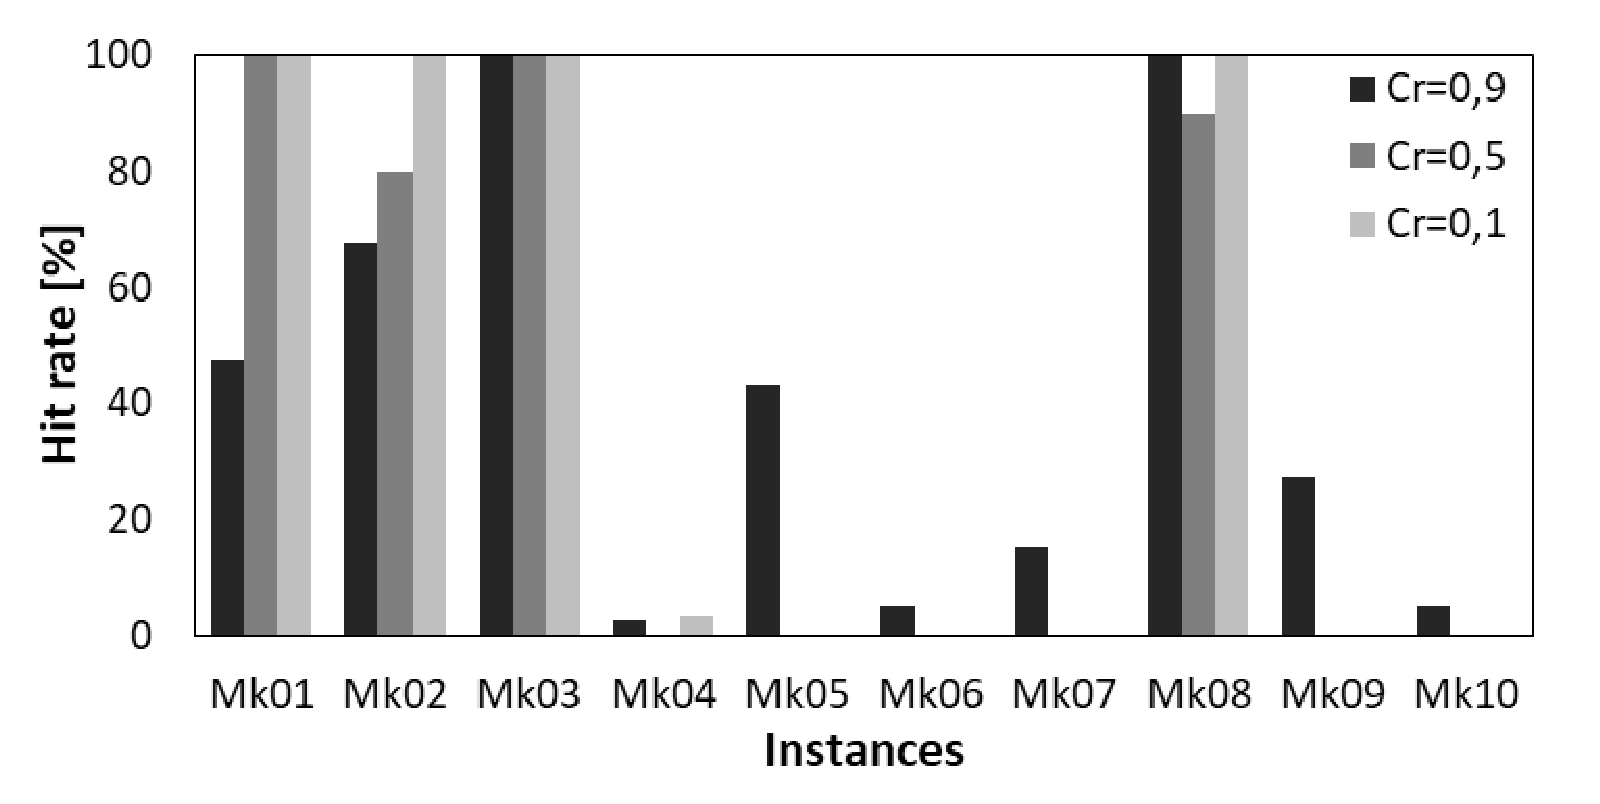
\includegraphics[width=0.75\textwidth]{figures/DE-hitRate.eps}
%    \caption{Hit Rate of the DE with different Cr values considering all FJSSP instances.}
%    \label{fig:DEhitRate}
%\end{minipage}  
%\hspace{0.5cm}
%\begin{minipage}[b]{0.5\linewidth}
%    \centering
%    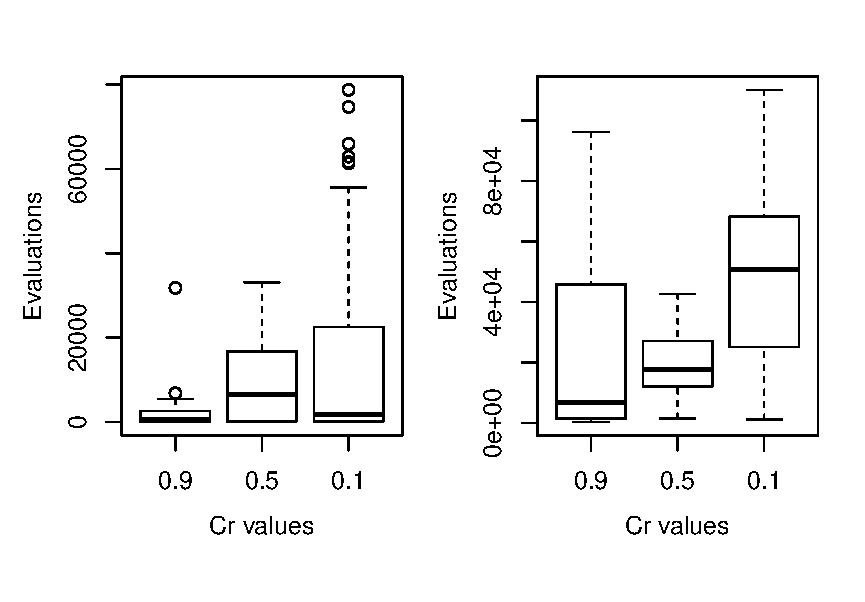
\includegraphics[width=0.75\textwidth]{figures/DE-Evaluations.eps}
%    \caption{Total number of evaluations done by running DE with different Cr values considering all FJSSP instances.}
%    \label{fig:DEevaluations}
%\end{minipage}
%\end{figure}


%\subsection{Results of the DE with Local Search}

Following analysis goes into detail of what happened with the introduction of a local search procedure to the DE algorithm (HDE) to solve the FJSSP. For that purpose, we considered three different $p_{LS}$ values: 0.1, 0.5 and 0.7 (low, medium, and high probability values), i.e. we study how the frequency of the LS application impacts on the DE performance.

Table~\ref{tab:HDE} shows the best and mean $C_{max}$ values obtained for the HDE with the different $p_{LS}$ values. The HDE algorithm applying the local search procedure with high frequency ($p_{LS}$=0.7) obtains low best $C_{max}$ values for the majority of the FJSSP instances. Moreover, this algorithm exhibits the lowest mean $C_{max}$ values for all instances. These indicate that the algorithm is able to find the optimum or the near-optimum values in the majority of the runs.  Moreover, the KW test indicates that there are statistical significant differences among the algorithms ($p$-values are lower than the level of significance). Comparing  $C_{max}$ values from Table~\ref{tab:resultsDE} and the ones from Table~\ref{tab:HDE}, we can observe that the HDE algorithms obtain best 

\begin{table}[!tb]
\scriptsize
\centering

\caption{$C_{max}$ values found by the HDE algorithm with different $p_{LS}$ values% for all FJSSP instances
.}
\begin{tabular}{|c|c|rrr|rrr|c|}
\hline
\multicolumn{1}{|c}{\multirow{2}{*}{Inst}} & \multicolumn{1}{|c}{\multirow{2}{*}{Opt.}} & \multicolumn{3}{|c}{Best $C_{max}$} & \multicolumn{3}{|c|}{Mean $C_{max}$ values $_{\pm}$ sd} &\multicolumn{1}{c|}{\multirow{2}{*}{KW}} \\
\cline{3-8}
\multicolumn{1}{|c}{} & \multicolumn{1}{|c|}{} &$p_{LS}$=0.1 & $p_{LS}$=0.5 & $p_{LS}$=0.7 & $p_{LS}$=0.1 & $p_{LS}$=0.5 & $p_{LS}$=0.7 & \multicolumn{1}{c|}{}\\
\hline
MK01 & 40 & \textbf{40} & \textbf{40} & \textbf{40} & 40.00  $_{\pm  0.00  }$ & 40.00  $_{\pm  0.00  }$ & 40.00  $_{\pm  0.00  }$ & -\\
MK02 & 26 & 27 & \textbf{26} & \textbf{26} & 27.00  $_{\pm  0.00  }$ & 26.80  $_{\pm  0.41  }$ & 26.77  $_{\pm  0.43  }$ & + \\
MK03 & 204 & \textbf{204} & \textbf{204} & \textbf{204} & 204.00  $_{\pm  0.00  }$ & 204.00  $_{\pm  0.00  }$ & 204.00  $_{\pm  0.00  }$ & - \\
MK04 & 60 & \textbf{60} & \textbf{60} & \textbf{60} & 61.20  $_{\pm  0.66  }$ & 60.33  $_{\pm  0.48  }$ & 60.17  $_{\pm  0.38  }$ & +\\
MK05 & 172 & 173 & 173 & 173 & 1.73  $_{\pm  0.18  }$ & 173.00  $_{\pm  0.00  }$ & 173.00  $_{\pm  0.00  }$ & +\\
MK06 & 58 & 62 & 61 & 60 & 63.27  $_{\pm  0.69  }$ & 62.13  $_{\pm  0.73  }$ & 61.90  $_{\pm  0.48  }$ & +\\
MK07 & 139 & 140 & \textbf{139} & 140 & 142.37  $_{\pm  0.96  }$ & 140.83  $_{\pm 0.79  }$ & 140.63  $_{\pm  0.61  }$ &+\\
MK08 & 523 & \textbf{523} & \textbf{523} & \textbf{523} & 523.00  $_{\pm 0.00  }$ & 523.00  $_{\pm  0.00  }$ & 523.00  $_{\pm  0.00  }$ &-\\
MK09 & 307 & \textbf{307} & \textbf{307} & \textbf{307} & 309.93  $_{\pm  1.53  }$ & 307.67  $_{\pm  1.06  }$ & 307.37  $_{\pm  0.89  }$ &+\\
MK10 & 197 & 225 & 223 & 219 & 228.20  $_{\pm  1.97  }$ & 225.77  $_{\pm  1.36  }$ & 224.73  $_{\pm  1.66 }$ &+\\
\hline
\end{tabular}
\label{tab:HDE}
\end{table}

%%%%%%%%

Figure~\ref{fig:HDEevaluations} illustrates the distribution of the number of evaluations to find the best $C_{max}$ values for the HDE algorithms with different $P_{LS}$ values. We observe that the HDE algorithm with $P_{LS}$=0.7 needs less number of evaluations than the rest of the algorithms. If we also consider the $C_{max}$ values obtained by each HDE, the one with $P_{LS}$=0.7 is the best approach to solve this problem.

\begin{figure}[!tb]
\scriptsize
\centering
%\begin{minipage}[b]{0.4\linewidth}
%    \centering
%    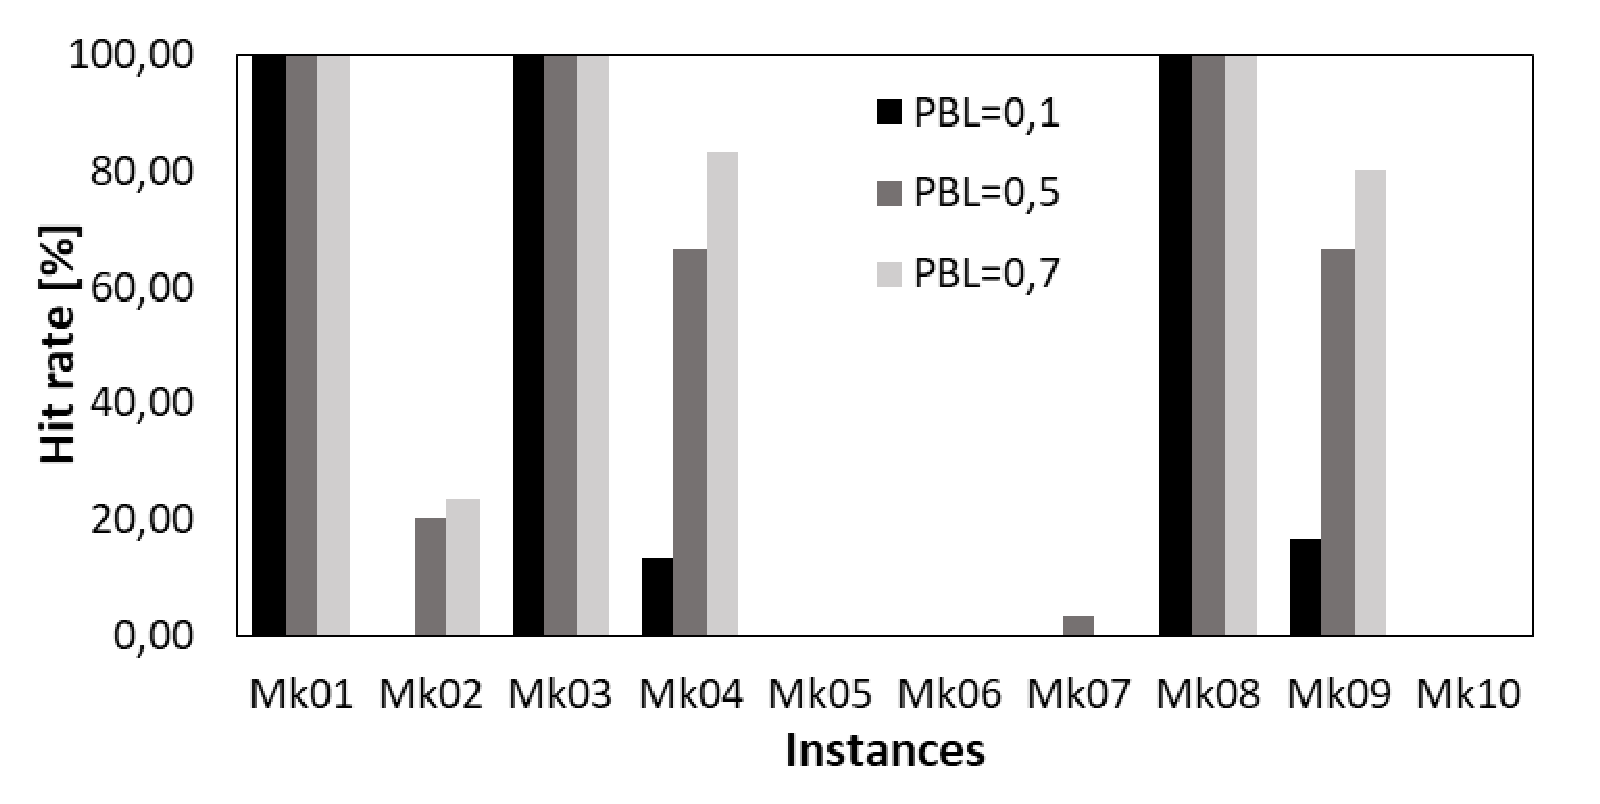
\includegraphics[width=\linewidth]{figures/DELS-hitRate.eps}
%    \caption{Hit Rate of the HDE with Different Cr values considering all FJSSP instances.}
%    \label{fig:DEhitRate}
%\end{minipage}
%\hspace{0.2cm}
\begin{minipage}[b]{0.4\linewidth}
    \centering
    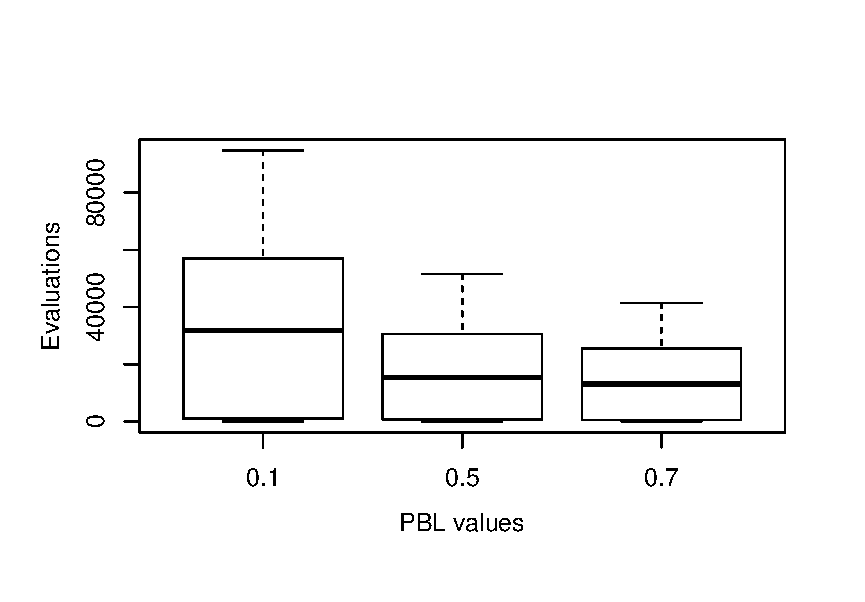
\includegraphics[width=\linewidth]{figures/DELS-Evaluations.eps}
    \vspace{-0.9cm}
    \caption{Total number of evaluations for the HDE %with different $P_{BL}$ values considering all FJSSP instances
    .}
    \label{fig:HDEevaluations}
\end{minipage}  
\hspace{0.5cm}
\begin{minipage}[b]{0.4\linewidth}
%\begin{figure}[!htb]
\scriptsize
\centering
   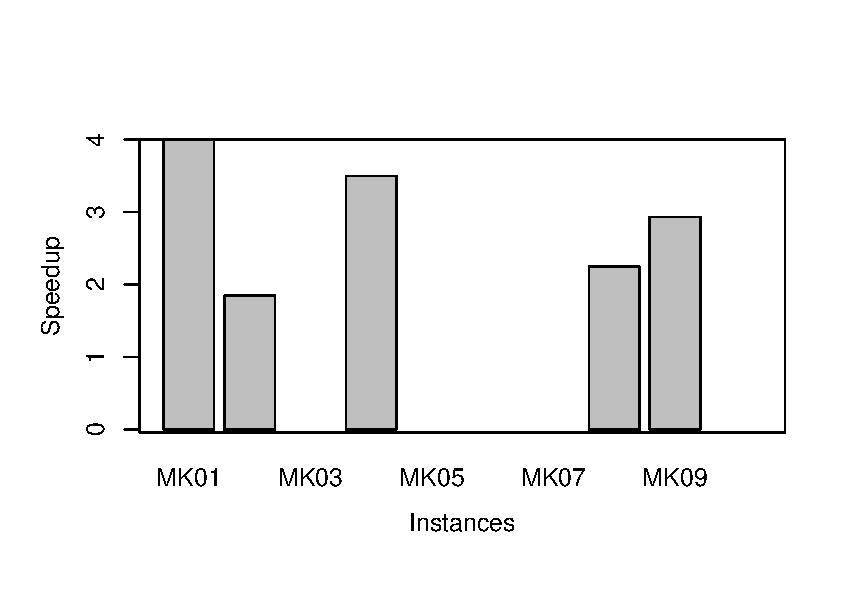
\includegraphics[width=\linewidth]{figures/speedup.eps}
   \vspace{-0.9cm}
    \caption{Speedup per FJSSP instances.}
    \label{fig:speedup}
%\end{figure}
\end{minipage}
\end{figure}


%\subsection{Results of the DE and parallelism}

%Finally, %in this section 
Following analysis is devoted to compare the HDE and its parallel version as described in Section~\ref{subsec:parallelHDE}. The most important measure of a parallel algorithm is the speedup. The speedup is defined as the ratio of the sequential execution time (HDE execution time, in this case) to the parallel execution time. For this analysis, we consider the weak speedup~\cite{albaMeta2005}. For that reason and following the best practice by Luque and Alba~\cite{Luque:2013:PGA:2564896}, the stopping criterion is based on the quality of the final solution achieved by the algorithms, which is set to the best known $C_{max}$ for each FJSSP instance (see column Opt of Table~\ref{tab:resultsDE}). Consequently, the speedup values is only reported  for the instances for which the HDE algorithm obtains the optimum value.%,as previously mentioned in previous sections.

%Once we established execution times of the HDE and the parallel HDE, we calculated the speedup values. 
Figure~\ref{fig:speedup} shows that the use of parallelization is worth while, which allow us to speed up the execution time with respect to the sequential HDE  near 3 times in average (the ideal speedup value is 4, the number of available cores per machine). 

Finally, to determine the goodness of the metaheuristics considered in this work, we present a comparison of the results from the HDE with several competitive algorithms present in the literature. This allows a comparative assessment of the algorithms for the FJSSP. In this comparison different population-based metaheuristics to solve the FJSSP are considered: i) a hybrid algorithm combining chaos particle swarm optimization with genetic algorithm (hGA)~\cite{tang2011}, ii) a bi-population based estimation of distribution algorithm (BEDA)~\cite{Wang2012917},  iii) an ant colony optimization (IACO)~\cite{WANG2017}, and finally, iv) a hybrid differential evolutionary algorithm~\cite{YUAN2013246}. From the comparison, the $C_{max}$ values of HDE are similar with the values of remaining algorithms, for the majority of the ten instances (a comparative table is no included due to lack of space). This observation suggests that the HDE developed in this work is a competitive algorithm to solve the FJSSP. Comparisons regarding computational effort are hard to be carried out because the majority of the works do not report number of evaluations. Consequently, the relative efficiency of referred algorithms are difficult to contrast in order to obtain meaningful comparisons.

\begin{table}[!tb]
\scriptsize
  \centering
  \caption{Comparison between HDE and population-based Metaheuristics from the literature}
    \begin{tabular}{l|rrrrrrrrrr|}
    \hline
    \multicolumn{1}{r}{} & \multicolumn{1}{l}{MK01} & \multicolumn{1}{l}{MK02} & \multicolumn{1}{l}{MK03} & \multicolumn{1}{l}{MK04} & \multicolumn{1}{l}{MK05} & \multicolumn{1}{l}{MK06} & \multicolumn{1}{l}{MK07} & \multicolumn{1}{l}{MK08} & \multicolumn{1}{l}{MK09} & \multicolumn{1}{l}{MK10} \\
    \hline
    HDE   & \textbf{40} & \textbf{26} & \textbf{204} & \textbf{60} & 173   & 60    & 140   & \textbf{523} & \textbf{307} & 219 \\
    hGA   & \textbf{40} & \textbf{26} & \textbf{204} & 62    & \textbf{172} & 65    & 140   & \textbf{523} & 310   & 214 \\
    BEDA  & \textbf{40} & \textbf{26} & \textbf{204} & \textbf{60} & \textbf{172} & 60    & \textbf{139} & \textbf{523} & \textbf{307} & 206 \\
    IACO  & \textbf{40} & \textbf{26} & \textbf{204} & \textbf{60} & 173   & 60    & 140   & \textbf{523} & \textbf{307} & 208 \\
    HDE   & \textbf{40} & \textbf{26} & \textbf{204} & \textbf{60} & \textbf{172} & \textbf{57} & \textbf{139} & \textbf{523} & \textbf{307} & \textbf{198} \\
\hline
    \end{tabular}%
  \label{tab:addlabel}%
\end{table}%


\section{Conclusions}
\vspace{-0.4cm}
In this article, we have presented a simple DE algorithm to solve the FJSSP. In
this study, the traditional real-parameter global optimizer is considered to maintain the properties of the DE in their natural configuration. The DE is enhanced with a very simple local search procedure, obtaining a hybrid DE (HDE). Moreover, each iteration of the DE is parallelised to speed up the computation. The results indicate that the HDE with a high probability, at which the local search procedure is applied, is able to find the best solutions for the FJSSP. Moreover, when HDE is contrasted with algorithms in the literature, it also becomes a competitive approach. As a consequence, HDE gives good solutions to this NP-hard problem in an efficient and competitive way.

As future research activities, we will plan to extend the study by including another set of instances with high dimensionality. Furthermore, variants of the FJSSP with more constraints will be evaluated considering the approaches developed in this article.

\section*{Acknowledgements}
\vspace{-0.4cm}
This research is is supported by Universidad Nacional de La Pampa, and the Incentive Program from MINCyT. The last author acknowledges CONICET.

\scriptsize
\bibliographystyle{IEEEtran}
\bibliography{fjsspBiblio}

\end{document}
        